
%% bare_jrnl_compsoc.tex
%% V1.3
%% 2007/01/11
%% by Michael Shell
%% See:
%% http://www.michaelshell.org/
%% for current contact information.
%%
%% This is a skeleton file demonstrating the use of IEEEtran.cls
%% (requires IEEEtran.cls version 1.7 or later) with an IEEE Computer
%% Society journal paper.
%%
%% Support sites:
%% http://www.michaelshell.org/tex/ieeetran/
%% http://www.ctan.org/tex-archive/macros/latex/contrib/IEEEtran/
%% and
%% http://www.ieee.org/

%%*************************************************************************
%% Legal Notice:
%% This code is offered as-is without any warranty either expressed or
%% implied; without even the implied warranty of MERCHANTABILITY or
%% FITNESS FOR A PARTICULAR PURPOSE! 
%% User assumes all risk.
%% In no event shall IEEE or any contributor to this code be liable for
%% any damages or losses, including, but not limited to, incidental,
%% consequential, or any other damages, resulting from the use or misuse
%% of any information contained here.
%%
%% All comments are the opinions of their respective authors and are not
%% necessarily endorsed by the IEEE.
%%
%% This work is distributed under the LaTeX Project Public License (LPPL)
%% ( http://www.latex-project.org/ ) version 1.3, and may be freely used,
%% distributed and modified. A copy of the LPPL, version 1.3, is included
%% in the base LaTeX documentation of all distributions of LaTeX released
%% 2003/12/01 or later.
%% Retain all contribution notices and credits.
%% ** Modified files should be clearly indicated as such, including  **
%% ** renaming them and changing author support contact information. **
%%
%% File list of work: IEEEtran.cls, IEEEtran_HOWTO.pdf, bare_adv.tex,
%%                    bare_conf.tex, bare_jrnl.tex, bare_jrnl_compsoc.tex
%%*************************************************************************

% *** Authors should verify (and, if needed, correct) their LaTeX system  ***
% *** with the testflow diagnostic prior to trusting their LaTeX platform ***
% *** with production work. IEEE's font choices can trigger bugs that do  ***
% *** not appear when using other class files.                            ***
% The testflow support page is at:
% http://www.michaelshell.org/tex/testflow/




% Note that the a4paper option is mainly intended so that authors in
% countries using A4 can easily print to A4 and see how their papers will
% look in print - the typesetting of the document will not typically be
% affected with changes in paper size (but the bottom and side margins will).
% Use the testflow package mentioned above to verify correct handling of
% both paper sizes by the user's LaTeX system.
%
% Also note that the "draftcls" or "draftclsnofoot", not "draft", option
% should be used if it is desired that the figures are to be displayed in
% draft mode.
%
% The Computer Society usually requires 12pt for submissions.
%
\documentclass[12pt,journal,compsoc]{IEEEtran}
%
% If IEEEtran.cls has not been installed into the LaTeX system files,
% manually specify the path to it like:
% \documentclass[12pt,journal,compsoc]{../sty/IEEEtran}





% Some very useful LaTeX packages include:
% (uncomment the ones you want to load)


% *** MISC UTILITY PACKAGES ***
%
%\usepackage{ifpdf}
% Heiko Oberdiek's ifpdf.sty is very useful if you need conditional
% compilation based on whether the output is pdf or dvi.
% usage:
% \ifpdf
%   % pdf code
% \else
%   % dvi code
% \fi
% The latest version of ifpdf.sty can be obtained from:
% http://www.ctan.org/tex-archive/macros/latex/contrib/oberdiek/
% Also, note that IEEEtran.cls V1.7 and later provides a builtin
% \ifCLASSINFOpdf conditional that works the same way.
% When switching from latex to pdflatex and vice-versa, the compiler may
% have to be run twice to clear warning/error messages.






% *** CITATION PACKAGES ***
%
\ifCLASSOPTIONcompsoc
  % IEEE Computer Society needs nocompress option
  % requires cite.sty v4.0 or later (November 2003)
  % \usepackage[nocompress]{cite}
\else
  % normal IEEE
  % \usepackage{cite}
\fi
% cite.sty was written by Donald Arseneau
% V1.6 and later of IEEEtran pre-defines the format of the cite.sty package
% \cite{} output to follow that of IEEE. Loading the cite package will
% result in citation numbers being automatically sorted and properly
% "compressed/ranged". e.g., [1], [9], [2], [7], [5], [6] without using
% cite.sty will become [1], [2], [5]--[7], [9] using cite.sty. cite.sty's
% \cite will automatically add leading space, if needed. Use cite.sty's
% noadjust option (cite.sty V3.8 and later) if you want to turn this off.
% cite.sty is already installed on most LaTeX systems. Be sure and use
% version 4.0 (2003-05-27) and later if using hyperref.sty. cite.sty does
% not currently provide for hyperlinked citations.
% The latest version can be obtained at:
% http://www.ctan.org/tex-archive/macros/latex/contrib/cite/
% The documentation is contained in the cite.sty file itself.
%
% Note that some packages require special options to format as the Computer
% Society requires. In particular, Computer Society  papers do not use
% compressed citation ranges as is done in typical IEEE papers
% (e.g., [1]-[4]). Instead, they list every citation separately in order
% (e.g., [1], [2], [3], [4]). To get the latter we need to load the cite
% package with the nocompress option which is supported by cite.sty v4.0
% and later. Note also the use of a CLASSOPTION conditional provided by
% IEEEtran.cls V1.7 and later.





% *** GRAPHICS RELATED PACKAGES ***
%
\ifCLASSINFOpdf
  % \usepackage[pdftex]{graphicx}
  % declare the path(s) where your graphic files are
  % \graphicspath{{../pdf/}{../jpeg/}}
  % and their extensions so you won't have to specify these with
  % every instance of \includegraphics
  % \DeclareGraphicsExtensions{.pdf,.jpeg,.png}
\else
  % or other class option (dvipsone, dvipdf, if not using dvips). graphicx
  % will default to the driver specified in the system graphics.cfg if no
  % driver is specified.
   %\usepackage[dvips]{graphicx}
   \usepackage[dvipdfmx]{graphicx}
  % declare the path(s) where your graphic files are
  % \graphicspath{{../eps/}}
  % and their extensions so you won't have to specify these with
  % every instance of \includegraphics
  % \DeclareGraphicsExtensions{.eps}
\fi
% graphicx was written by David Carlisle and Sebastian Rahtz. It is
% required if you want graphics, photos, etc. graphicx.sty is already
% installed on most LaTeX systems. The latest version and documentation can
% be obtained at: 
% http://www.ctan.org/tex-archive/macros/latex/required/graphics/
% Another good source of documentation is "Using Imported Graphics in
% LaTeX2e" by Keith Reckdahl which can be found as epslatex.ps or
% epslatex.pdf at: http://www.ctan.org/tex-archive/info/
%
% latex, and pdflatex in dvi mode, support graphics in encapsulated
% postscript (.eps) format. pdflatex in pdf mode supports graphics
% in .pdf, .jpeg, .png and .mps (metapost) formats. Users should ensure
% that all non-photo figures use a vector format (.eps, .pdf, .mps) and
% not a bitmapped formats (.jpeg, .png). IEEE frowns on bitmapped formats
% which can result in "jaggedy"/blurry rendering of lines and letters as
% well as large increases in file sizes.
%
% You can find documentation about the pdfTeX application at:
% http://www.tug.org/applications/pdftex





% *** MATH PACKAGES ***
%
%\usepackage[cmex10]{amsmath}
% A popular package from the American Mathematical Society that provides
% many useful and powerful commands for dealing with mathematics. If using
% it, be sure to load this package with the cmex10 option to ensure that
% only type 1 fonts will utilized at all point sizes. Without this option,
% it is possible that some math symbols, particularly those within
% footnotes, will be rendered in bitmap form which will result in a
% document that can not be IEEE Xplore compliant!
%
% Also, note that the amsmath package sets \interdisplaylinepenalty to 10000
% thus preventing page breaks from occurring within multiline equations. Use:
%\interdisplaylinepenalty=2500
% after loading amsmath to restore such page breaks as IEEEtran.cls normally
% does. amsmath.sty is already installed on most LaTeX systems. The latest
% version and documentation can be obtained at:
% http://www.ctan.org/tex-archive/macros/latex/required/amslatex/math/





% *** SPECIALIZED LIST PACKAGES ***
%
%\usepackage{algorithmic}
% algorithmic.sty was written by Peter Williams and Rogerio Brito.
% This package provides an algorithmic environment fo describing algorithms.
% You can use the algorithmic environment in-text or within a figure
% environment to provide for a floating algorithm. Do NOT use the algorithm
% floating environment provided by algorithm.sty (by the same authors) or
% algorithm2e.sty (by Christophe Fiorio) as IEEE does not use dedicated
% algorithm float types and packages that provide these will not provide
% correct IEEE style captions. The latest version and documentation of
% algorithmic.sty can be obtained at:
% http://www.ctan.org/tex-archive/macros/latex/contrib/algorithms/
% There is also a support site at:
% http://algorithms.berlios.de/index.html
% Also of interest may be the (relatively newer and more customizable)
% algorithmicx.sty package by Szasz Janos:
% http://www.ctan.org/tex-archive/macros/latex/contrib/algorithmicx/




% *** ALIGNMENT PACKAGES ***
%
%\usepackage{array}
% Frank Mittelbach's and David Carlisle's array.sty patches and improves
% the standard LaTeX2e array and tabular environments to provide better
% appearance and additional user controls. As the default LaTeX2e table
% generation code is lacking to the point of almost being broken with
% respect to the quality of the end results, all users are strongly
% advised to use an enhanced (at the very least that provided by array.sty)
% set of table tools. array.sty is already installed on most systems. The
% latest version and documentation can be obtained at:
% http://www.ctan.org/tex-archive/macros/latex/required/tools/


%\usepackage{mdwmath}
%\usepackage{mdwtab}
% Also highly recommended is Mark Wooding's extremely powerful MDW tools,
% especially mdwmath.sty and mdwtab.sty which are used to format equations
% and tables, respectively. The MDWtools set is already installed on most
% LaTeX systems. The lastest version and documentation is available at:
% http://www.ctan.org/tex-archive/macros/latex/contrib/mdwtools/


% IEEEtran contains the IEEEeqnarray family of commands that can be used to
% generate multiline equations as well as matrices, tables, etc., of high
% quality.


%\usepackage{eqparbox}
% Also of notable interest is Scott Pakin's eqparbox package for creating
% (automatically sized) equal width boxes - aka "natural width parboxes".
% Available at:
% http://www.ctan.org/tex-archive/macros/latex/contrib/eqparbox/





% *** SUBFIGURE PACKAGES ***
\ifCLASSOPTIONcompsoc
\usepackage[tight,normalsize,sf,SF]{subfigure}
\else
\usepackage[tight,footnotesize]{subfigure}
\fi
% subfigure.sty was written by Steven Douglas Cochran. This package makes it
% easy to put subfigures in your figures. e.g., "Figure 1a and 1b". For IEEE
% work, it is a good idea to load it with the tight package option to reduce
% the amount of white space around the subfigures. Computer Society papers
% use a larger font and \sffamily font for their captions, hence the
% additional options needed under compsoc mode. subfigure.sty is already
% installed on most LaTeX systems. The latest version and documentation can
% be obtained at:
% http://www.ctan.org/tex-archive/obsolete/macros/latex/contrib/subfigure/
% subfigure.sty has been superceeded by subfig.sty.


%\ifCLASSOPTIONcompsoc
%  \usepackage[caption=false]{caption}
%  \usepackage[font=normalsize,labelfont=sf,textfont=sf]{subfig}
%\else
%  \usepackage[caption=false]{caption}
%  \usepackage[font=footnotesize]{subfig}
%\fi
% subfig.sty, also written by Steven Douglas Cochran, is the modern
% replacement for subfigure.sty. However, subfig.sty requires and
% automatically loads Axel Sommerfeldt's caption.sty which will override
% IEEEtran.cls handling of captions and this will result in nonIEEE style
% figure/table captions. To prevent this problem, be sure and preload
% caption.sty with its "caption=false" package option. This is will preserve
% IEEEtran.cls handing of captions. Version 1.3 (2005/06/28) and later 
% (recommended due to many improvements over 1.2) of subfig.sty supports
% the caption=false option directly:
%\ifCLASSOPTIONcompsoc
%  \usepackage[caption=false,font=normalsize,labelfont=sf,textfont=sf]{subfig}
%\else
%  \usepackage[caption=false,font=footnotesize]{subfig}
%\fi
%
% The latest version and documentation can be obtained at:
% http://www.ctan.org/tex-archive/macros/latex/contrib/subfig/
% The latest version and documentation of caption.sty can be obtained at:
% http://www.ctan.org/tex-archive/macros/latex/contrib/caption/




% *** FLOAT PACKAGES ***
%
%\usepackage{fixltx2e}
% fixltx2e, the successor to the earlier fix2col.sty, was written by
% Frank Mittelbach and David Carlisle. This package corrects a few problems
% in the LaTeX2e kernel, the most notable of which is that in current
% LaTeX2e releases, the ordering of single and double column floats is not
% guaranteed to be preserved. Thus, an unpatched LaTeX2e can allow a
% single column figure to be placed prior to an earlier double column
% figure. The latest version and documentation can be found at:
% http://www.ctan.org/tex-archive/macros/latex/base/



%\usepackage{stfloats}
% stfloats.sty was written by Sigitas Tolusis. This package gives LaTeX2e
% the ability to do double column floats at the bottom of the page as well
% as the top. (e.g., "\begin{figure*}[!b]" is not normally possible in
% LaTeX2e). It also provides a command:
%\fnbelowfloat
% to enable the placement of footnotes below bottom floats (the standard
% LaTeX2e kernel puts them above bottom floats). This is an invasive package
% which rewrites many portions of the LaTeX2e float routines. It may not work
% with other packages that modify the LaTeX2e float routines. The latest
% version and documentation can be obtained at:
% http://www.ctan.org/tex-archive/macros/latex/contrib/sttools/
% Documentation is contained in the stfloats.sty comments as well as in the
% presfull.pdf file. Do not use the stfloats baselinefloat ability as IEEE
% does not allow \baselineskip to stretch. Authors submitting work to the
% IEEE should note that IEEE rarely uses double column equations and
% that authors should try to avoid such use. Do not be tempted to use the
% cuted.sty or midfloat.sty packages (also by Sigitas Tolusis) as IEEE does
% not format its papers in such ways.




%\ifCLASSOPTIONcaptionsoff
%  \usepackage[nomarkers]{endfloat}
% \let\MYoriglatexcaption\caption
% \renewcommand{\caption}[2][\relax]{\MYoriglatexcaption[#2]{#2}}
%\fi
% endfloat.sty was written by James Darrell McCauley and Jeff Goldberg.
% This package may be useful when used in conjunction with IEEEtran.cls'
% captionsoff option. Some IEEE journals/societies require that submissions
% have lists of figures/tables at the end of the paper and that
% figures/tables without any captions are placed on a page by themselves at
% the end of the document. If needed, the draftcls IEEEtran class option or
% \CLASSINPUTbaselinestretch interface can be used to increase the line
% spacing as well. Be sure and use the nomarkers option of endfloat to
% prevent endfloat from "marking" where the figures would have been placed
% in the text. The two hack lines of code above are a slight modification of
% that suggested by in the endfloat docs (section 8.3.1) to ensure that
% the full captions always appear in the list of figures/tables - even if
% the user used the short optional argument of \caption[]{}.
% IEEE papers do not typically make use of \caption[]'s optional argument,
% so this should not be an issue. A similar trick can be used to disable
% captions of packages such as subfig.sty that lack options to turn off
% the subcaptions:
% For subfig.sty:
% \let\MYorigsubfloat\subfloat
% \renewcommand{\subfloat}[2][\relax]{\MYorigsubfloat[]{#2}}
% For subfigure.sty:
% \let\MYorigsubfigure\subfigure
% \renewcommand{\subfigure}[2][\relax]{\MYorigsubfigure[]{#2}}
% However, the above trick will not work if both optional arguments of
% the \subfloat/subfig command are used. Furthermore, there needs to be a
% description of each subfigure *somewhere* and endfloat does not add
% subfigure captions to its list of figures. Thus, the best approach is to
% avoid the use of subfigure captions (many IEEE journals avoid them anyway)
% and instead reference/explain all the subfigures within the main caption.
% The latest version of endfloat.sty and its documentation can obtained at:
% http://www.ctan.org/tex-archive/macros/latex/contrib/endfloat/
%
% The IEEEtran \ifCLASSOPTIONcaptionsoff conditional can also be used
% later in the document, say, to conditionally put the References on a 
% page by themselves.




% *** PDF, URL AND HYPERLINK PACKAGES ***
%
%\usepackage{url}
% url.sty was written by Donald Arseneau. It provides better support for
% handling and breaking URLs. url.sty is already installed on most LaTeX
% systems. The latest version can be obtained at:
% http://www.ctan.org/tex-archive/macros/latex/contrib/misc/
% Read the url.sty source comments for usage information. Basically,
% \url{my_url_here}.

\hyphenation{op-tical net-works semi-conduc-tor}


\begin{document}
\title{Bare Demo of IEEEtran.cls\\ for Computer Society Journals}
\author{
Yusuke~Fujii,~\IEEEmembership{Member,~IEEE,}
Takuya~Azumi,~\IEEEmembership{Member,~IEEE,}
Nobuhiko~Nishio,~\IEEEmembership{Member,~IEEE,}
Shinpei~Kato,~\IEEEmembership{Member,~IEEE,}
\IEEEcompsocitemizethanks{
\IEEEcompsocthanksitem Y. Fujii is with the College of Information Science and Engineering, Ritsumeikan University, Shiga, Kusatsu Noji-higashi, 1-1-1 Japan
\IEEEcompsocthanksitem T. Azumi is with the Graduate School of Information Science and Engineering, Osaka University,Japan
\IEEEcompsocthanksitem N. Nishio is with the Graduate School of Engineering Science, Ritsumeikan University, Shiga, Kusatsu Noji-higashi, 1-1-1 Japan
\IEEEcompsocthanksitem S. Kato is with the School of Information Science, Nagoya University
}}

% The paper headers
\markboth{Journal of \LaTeX\ Class Files,~Vol.~6, No.~1, January~2007}%
{Shell \MakeLowercase{\textit{et al.}}: Bare Demo of IEEEtran.cls for Computer Society Journals}
% The only time the second header will appear is for the odd numbered pages
% after the title page when using the twoside option.
% 
% *** Note that you probably will NOT want to include the author's ***
% *** name in the headers of peer review papers.                   ***
% You can use \ifCLASSOPTIONpeerreview for conditional compilation here if
% you desire.



% The publisher's ID mark at the bottom of the page is less important with
% Computer Society journal papers as those publications place the marks
% outside of the main text columns and, therefore, unlike regular IEEE
% journals, the available text space is not reduced by their presence.
% If you want to put a publisher's ID mark on the page you can do it like
% this:
%\IEEEpubid{0000--0000/00\$00.00~\copyright~2007 IEEE}
% or like this to get the Computer Society new two part style.
%\IEEEpubid{\makebox[\columnwidth]{\hfill 0000--0000/00/\$00.00~\copyright~2007 IEEE}%
%\hspace{\columnsep}\makebox[\columnwidth]{Published by the IEEE Computer Society\hfill}}
% Remember, if you use this you must call \IEEEpubidadjcol in the second
% column for its text to clear the IEEEpubid mark (Computer Society jorunal
% papers don't need this extra clearance.)



% use for special paper notices
%\IEEEspecialpapernotice{(Invited Paper)}



% for Computer Society papers, we must declare the abstract and index terms
% PRIOR to the title within the \IEEEcompsoctitleabstractindextext IEEEtran
% command as these need to go into the title area created by \maketitle.
\IEEEcompsoctitleabstractindextext{%
\begin{abstract}
%\boldmath
The abstract goes here.
\end{abstract}
% IEEEtran.cls defaults to using nonbold math in the Abstract.
% This preserves the distinction between vectors and scalars. However,
% if the journal you are submitting to favors bold math in the abstract,
% then you can use LaTeX's standard command \boldmath at the very start
% of the abstract to achieve this. Many IEEE journals frown on math
% in the abstract anyway. In particular, the Computer Society does
% not want either math or citations to appear in the abstract.

% Note that keywords are not normally used for peerreview papers.
\begin{IEEEkeywords}
Computer Society, IEEEtran, journal, \LaTeX, paper, template.
\end{IEEEkeywords}}


% make the title area
\maketitle


% To allow for easy dual compilation without having to reenter the
% abstract/keywords data, the \IEEEcompsoctitleabstractindextext text will
% not be used in maketitle, but will appear (i.e., to be "transported")
% here as \IEEEdisplaynotcompsoctitleabstractindextext when compsoc mode
% is not selected <OR> if conference mode is selected - because compsoc
% conference papers position the abstract like regular (non-compsoc)
% papers do!
\IEEEdisplaynotcompsoctitleabstractindextext
% \IEEEdisplaynotcompsoctitleabstractindextext has no effect when using
% compsoc under a non-conference mode.


% For peer review papers, you can put extra information on the cover
% page as needed:
% \ifCLASSOPTIONpeerreview
% \begin{center} \bfseries EDICS Category: 3-BBND \end{center}
% \fi
%
% For peerreview papers, this IEEEtran command inserts a page break and
% creates the second title. It will be ignored for other modes.
\IEEEpeerreviewmaketitle



\section{Introduction}
\IEEEPARstart{R}{eal-time} system $B$O<R2q%$%s%U%i$K$*$$$F=EMW$JLr3d$rC4$C$F$$$k!#(B
Real-time systems$B$O$3$l$^$G$b!"%m%\%C%H$d%^%k%A%a%G%#%"%7%9%F%`!"9)>l%7%9%F%`$J$I<R2q$KL)@\$K4X$o$k%7%9%F%`$H$7$F!"(B
$BLr3d$r2L$?$7$F$-$?!#(B
$B$5$i$K$3$l$+$i$O!"(BCyber-physical system$B$H$$$&9M$(J}$,H/C#$7$F$-$F$*$j!"$h$j<R2q$r;Y$($F$$$/%$%s%U%i$H$7$FLr3d$rC4$C$F$$$/$H9M$($F$$$k!#(B
Cyber-Physial systems represent next generation networked and embedded systems.
These system was tightly coupled with computation and physical elements to control real-world phenomena.
There control algorithms are becoming more and more complex, which distinguishes CPS from traditional safety-critical embedded systems in terms of the computational cost.
From their factors, CPS requires more high-performance computing resources to achieve real-fast computing.

One solution for achieving real-fast computing is to use GPUs.
GPUs can be realized fast computing for data-intensive application by parallel computing wiht many-core processor.
GPUs application developing is become easier since vendor was official supported GPGPU framework that is include programming language and runtime.
So GPUs have been rapidly spread.

$B$5$i$K6C$/$3$H$K(BGPU$B5;=Q$OH/E82DG=@-$,9b$$!#(B
2013$BG/$KH/I=$5$l!"$=$N@-G=$+$iOCBj$K$J$C$?(BNVIDIA$B$N(BGeforce GTX TITAN$B$NC1@:EYIbF0>.?tE@1i;;@-G=$O(B4.5TFLOPS$B$G$"$k$,!"(B2014$BG/$KH/I=$5$l$?(BGeforce GTX TITAN Z$B$O(B8T Flops$B$N@-G=$r;}$C$F$$$k!#$3$N@.D9N($O0[>o$H$$$C$F$b2a8@$G$O$J$$!#(B
$B2C$($F(BGPU$B$H$$$($PBgNL$N%3%"$,Ek:\$5$l$F$$$k$3$H$+$i!"D>46E*$K$OEENO>CHq$,7c$7$$$H;W$o$l$F$$$k!#(B
$B$7$+$7$J$,$iG=NO$"$?$j$NEENO>CHq$O=>Mh$N(BCPU$B$KHf$Y$F$+$J$jM%$l$F$*$j!"(B
CPS$B$N%K!<%:$r@dL/$KK~$?$7$F$$$k$H$$$(!"<B:]$N%"%W%j%1!<%7%g%s$G$b(BGPU$B$OMxMQ$5$l$F$$$k!#(B
$BNc$($P(BObject detection, pedestrian tracking, navigation and route plannning.

GPU$B$GHFMQ7W;;$9$k$3$H$r(BGeneral Purpose GPU (GPGPU) $B$H8F$V(B.
GPGPU$B$OG!2?$J$k4D6-$G$bF0:n$9$k$H$$$&$3$H$G$O$J$/$$$/$D$+$N@)8B$,$"$k!#(B
$B%O!<%I%&%'%"$,Ek:\$G$-$k$+$H$$$&E@$OEvA3$H$7$F!"(B
$B%Y%s%@!<$K$h$C$F%i%$%V%i%j$d%G%P%$%9%I%i%$%P$J$I$N%i%s%?%$%`$,Ds6!$5$l$k4D6-$N$_$GF0:n2DG=$G$"$k!#(B
$B8=>u%Y%s%@!<$K$h$C$F(BGPGPU$B$,%5%]!<%H$5$l$F$$$k$N$O(BWindows$B!"(BMac OSX$B!"(BLinux$B$N$_$G$"$k!#(B
Linux$B$N%a%$%s%i%$%s$G$O(BSCHED\_DEADLINE$B$d(BPREEMPT\_RT$B$N$h$&$J(B
$B%j%"%k%?%$%`$J%o!<%/%m!<%I$r%5%]!<%H$9$k$?$a$N<h$jAH$_$,9T$o$l$F$$$k!#(B
$B2C$($F!"(BLinux$B$NJQ0[BN$H$7$F(BRTOS$B$H$7$FDs6!$5$l$F$$$k$b$N$b?tB?$/$"$j!"(B
$B%j%"%k%?%$%`$K:G$b6a$$$H8@$($k!#(B
$B$=$N$?$a!"K\O@J8$G$O(BLinux$B$rMQ$$$k!#(B

$B2f!9$NCN$k8B$j!"8=CJ3,$G:G$bM%$l$F$$$k$G$"$m$&(BGPU$B;q8;4IM}$K4X$9$k8&5f$O!"(B
GPUSync\cite{}$B$H(BGdev$B$G$"$j!"%j%"%k%?%$%`$K4X$7$F$O(BGPUSync$B$,0lJb@h$s$8$F$$$k!#(B
$B$7$+$7$J$,$i!"(BGPUSync$B$O(B$LITMUS^{RT}$$B>e$K<BAu$5$l$F$*$j!"%+!<%M%k$X$NJQ99$rB?J,$K4^$s$G$$$k!#(B
Gdev$B$K$D$$$F$b!"%G%P%$%9%I%i%$%P$N(BISR$B$KJQ99$r2C$($F$*$j!"(BOS$B$X$N%Q%C%A$r$"$F$k$3$H$G$N%$%s%9%H%l!<%7%g%s$rI,MW$H$7$F$$$k!#(B
$B$3$N%Q%C%A$rEv$F$k:n6H$O3+H/<T$H%f!<%6$XBg$-$JIiC4$rM?$($k!#(B
$B3+H/<T$O!">o$K:G?7$N%+!<%M%k$N%j%j!<%9$KDI$$IU$/$?$a$K!"%Q%C%A$r0];}$7$F$$$/5AL3$,$"$k!#(B
$B$7$+$7(BLinux$B$O$=$N99?7IQEY$,Aa$/!"3+H/<T$,:G?7$N%+!<%M%k$K$`$1$F%]!<%F%#%s%0:n6H$r40N;$5$;$kA0$K!"?7$7$$%P!<%8%g%s$N%j%j!<%9$,5/$-$k$3$H$,B?$$!#(B
$B$=$N$?$a%+!<%M%k$NA*Br$K$D$$$F@)8B$5$l$k798~$,$"$k!#(B


\textbf{Contribution:}
$BK\O@J8$G$O!"(BGPU$B$rJ];}$9$k%7%9%F%`$K$*$$$F!"%j%"%k%?%$%`$J%o!<%/%m!<%I$r%5%]!<%H$9$k$?$a$K!"%f!<%6!<%l%Y%k$G2DG=$J$3$H$r(BExplore$B$9$k!#(B
$B$3$3$G$N%f!<%6!<%l%Y%k$H$O!"(BOS$B$r$$$8$i$:$K%f!<%6$,$G$-$k$3$H$H$$$&0U$G$"$k!#(B

$B2f!9$O$3$l$^$G$K!"%+!<%M%k$K%Q%C%A$rEv$F$:$K!"%f!<%6%l%Y%k$G(BRTOS$B3HD%$,<B8=2DG=$J(BRESCH\cite{}$B$rDs0F$7$F$-$?!#(B
RESCH$B$O(BLinux$B$N%m!<%@%V%k%+!<%M%k%b%8%e!<%k$rMxMQ$7$F$*$j!"%+!<%M%k$NFbIt4X?t$rMxMQ$7$F%9%1%8%e!<%j%s%0$9$k$3$H$G!"%f!<%6%l%Y%k$G$N%9%1%8%e!<%j%s%03HD%$r<B8=$7$F$$$k!#(B

$B;DG0$J$3$H$K!"(BRESCH$B$O0lHLE*$J(BCPU$B$G9=@.$5$l$?%7%9%F%`$rA[Dj$H$7$F:n$i$l$F$*$j!"(B
GPU$B$N$h$&$J%3%W%m%;%C%5$rDI2C$7$?%X%F%m%8%K%"%9$J4D6-$K$OBP1~$G$-$F$*$i$:!"(BCPS$B$N4pHW$H$7$FMQ$$$k$3$H$,$G$-$J$$!#(B

$B$7$+$7$J$,$i(BGPGPU$B%i%s%?%$%`$O%/%m!<%:%I%=!<%9$G$"$k!#(B




$BK\%"%W%m!<%A$O(BGPU$B$N%"%/%;%9$ND4Dd$d!"(BGPU$B%+!<%M%k=*N;;~$NF14|$N%O%s%I%j%s%0$r9T$$!"(BGPU$B$N%9%1%8%e!<%j%s%0$r2DG=$H$7$?>e$G!"(BRESCH$B$N%"%W%m!<%A$K:\$;$F%f!<%6%l%Y%k$G(BGPU$B$N%9%1%8%e!<%j%s%0$r%5%]!<%H$9$k!#(B
$B6qBNE*$K$O!"(B

$B2C$($F!"(BCPU$B$N$_$N%?%9%/$H(BGPU$B$,4^$^$l$k%?%9%/$,:.:_$9$k%7%9%F%`$K$*$$$F!"(B
$B9M$($i$l$k%9%1%8%e!<%j%s%0$N;EJ}$K$D$$$F9M;!$7!"$=$l$i$r<h<NA*Br$G$-$k4pHW$H$7$FDs6!$7$F$$$/$3$H$G!":#8e$N8&5fH/E8$K$D$J$2$F$$$/!#(B

\textbf{Organization}
This paper rest of 
$BK\O@J8$O"~>O$G9=@.$5$l$k!#(B
$B<!>O$G$O!"BP>]$H$9$k%7%9%F%`$N@bL@!#(B
3$B>O$G$O!"@h9T8&5f$r2r@b$7!"2r7h$9$Y$-E@$rNs5s$7!"(B
4$B>O$K$*$$$F$=$l$i$NE@$N2r7h$K$D$$$F@bL@$9$k!#(B
5$B>O$G$O!"(BLinux-RTXG$B$rMxMQ$7$?:]$N3F%*!<%P%X%C%I$K$D$$$F7WB,$7I>2A$r9T$&!#(B
6$B>O$GK\(BLinux-RTXG$B$NLdBjE@$H:#8e$NE8K>$K$D$$$F9M;!$7$F$$$/!#(B


\section{GPU Scheduling Discussion}
$B:#2s%?!<%2%C%H$H$9$k%7%9%F%`$O!"(B
$B0l8D0J>e$N(BCPU$B$,$"$j!"0l8D0J>e$N(BGPU$B$,Ek:\$5$l$?!"C10l$N%N!<%I$G$"$k!#(B
$B$=$N>e$G(BCPU$B$N$_$r;H$&%?%9%/!"(BGPU$B$r;H$&%?%9%/$,:.:_$7!"$=$l$>$l<~4|%?%9%/!"Hs<~4|%?%9%/$,B8:_$9$k$3$H$rA[Dj$9$k!#(B

Gdev$B$O2f!9$,Ds0F$7$F$-$?%*!<%W%s%=!<%9(BGPU$B%U%l!<%`%o!<%/$G$"$k!#(B
$B%j%6%Y!<%7%g%s%Y!<%9$N(BBAND$B%9%1%8%e!<%j%s%0$r9T$&$3$H$G%"%$%=%l!<%7%g%s$r3NJ]$7!"(BQoS$B$NC4J]$r9T$C$F$$$k!#(BBAND$B%9%1%8%e!<%i$O2>A[(BGPU$B$H$$$&7A$G%j%=!<%9$rJ,3d$7$F$*$j!"%?%9%/$O$=$l$>$l$N2>A[(BGPU$B$K=jB0$7$F$=$N%j%=!<%9$rMxMQ$7$F$$$/!#2>A[(BGPU$BFb$G$O(BFixed-Priority$B$K$h$C$F%9%1%8%e!<%k$5$l$k3,AXE*%9%1%8%e!<%i$N7A$r$H$C$F$$$k!#(B
Gdev$B$O%9%1%8%e!<%j%s%0$r(BGPU$B$X$N%"%/%;%93+;O$+$i!"F14|$9$k$^$G$H$7$F$*$j!"(BCPU$B$NF0:n$K0l@Z4XM?$7$F$$$J$$!#(B
Gdev's scheduling target is between the starting of GPU access and the synchronization.
It is not involved at all with the operation of CPU.

GPUSync$B$O!"(BElliot et al. $B$,Ds0F$9$k%j%"%k%?%$%`(BGPU$B%U%l!<%`%o!<%/$G$"$k!#(B
GPUSync$B$G$O(BGPU$B$N%9%1%8%e!<%j%s%0$G$O$J$/!"(BGPU$B$,4^$^$l$?%?%9%/$H$7$F%9%1%8%e!<%j%s%0$r9T$C$F$*$j!"(B
$BI>2A$G$O!"(BClustered-EDF$B$rMQ$$$?$3$H$r<($7$F$$$k!#(B
GPU$B$X$N%"%/%;%9$K$D$$$F$O(BBudget Enforcement$BJ}<0(B


\subsection{limitation}

\section{Linux-RTXG}

\subsection{GPU synchronization}
GPU$B$N%"%W%j%1!<%7%g%s$K$O6&DL$9$kFC@-$,$"$k!#(B
$B$=$l$O(BGPU$B$K=hM}$rH/9T$7$F$+$i!"=*N;$9$k$^$G$NBT5!;~4V$,H/@8$9$k$3$H$G$"$k!#(B
$BBT5!Cf$KF10l%?%9%/$G=hM}$r7QB3$9$kNc$b$"$k$,!"$=$N=hM}7k2L$OF14|$7$J$1$l$P<u$1<h$k$3$H$,$G$-$J$$$?$a!"(B
$BI,$:F14|;~4V$,H/@8$9$k!#(B
$B$3$NF14|;~4V$O(Bself-suspending$B$K4XO"$9$kLdBj$rH/@8$5$;$k!#(B
$B2C$($F!"$=$NF14|J}K!$K$h$C$F$O%l%$%F%s%7$,BgI}$KA}2C$9$k$?$a$K!"(B
$BE,@Z$J<jK!$K$h$C$FF14|$,9T$o$l$J$1$l$P$J$i$J$$!#(B

GPU$B$NF14|$O(B2$B$D$N<jK!$,$"$k!#(B
$B0l$D$O(Bfence$B$rMQ$$$kJ}K!!#(B
$B$b$&0l$D$O3d9~$_$rMQ$$$kJ}K!$G$"$k!#(B
GPU$B$K$OB?$/$N%(%s%8%s!J%^%$%/%m%3%s%H%m!<%i!K$,Ek:\$5$l$F$$$k!#(B
$BK\O@J8$G$O>\$7$$%"!<%-%F%/%A%c$OK\Bj$G$O$J$$$N$G>JN,$9$k!#>\:Y$O2a5n$NJ88%(B\cite{timegraph,fucc}$B$K5-:\$7$F$$$^$9!#(B
$B$3$N%(%s%8%s$K$O(BCOMPUTE$B$d(BCOPY$BMQ$N$b$N$,$"$k!#(B
$B$3$l$i$N%(%s%8%s$K$O%3%^%s%I%P%C%U%!$K3JG<$5$l$?%3%^%s%I$r(BFIFO$B$G=hM}$7$F$$$/!#(B
Fence$B$rMQ$$$?J}<0$G$O!"$^$:F14|MQ$K2>A[%"%I%l%96u4V$K%^%C%W$5$l$?%P%C%U%!$r(BGPU$B%a%b%j$KMQ0U$9$k!#(B
$B$=$7$F!"$3$N%a%b%j$KCM$r(BEngine$B7PM3$G=q$-9~$`MQ$K%3%^%s%I$rH/9T$9$k!#(B
$B$9$k$H!"%+!<%M%k<B9T$H%a%b%jE>Aw=*N;8e$K%(%s%8%s$,CM$r=q$-9~$`$?$a!"(B
CPU$BB&$G$=$N%^%C%W$5$l$?%a%b%j%"%I%l%9$r%]!<%j%s%0$7$J$,$i%A%'%C%/$9$l$PF14|$,2DG=$G$"$k!#(B
$B3d9~$_$rMQ$$$kJ}<0$K$D$$$F$b(BEngine$B$N5!G=$rMxMQ$9$k!#(B
$B%?%9%/$O(BTASK\_INTERRUPTIBLE/TASK\_UNINTERRUPTIBLE$B$K$7$?>e$G(Bschedule()$B$r8F$V$+!"(B
waitqueue$B$J$I$rMQ$$$F>e5-$KAjEv$9$k=hM}$r9T$$(Bsuspend$B$9$k!#(B
$B$=$7$F(BEngine$B$+$i3d9~$_$rH/@8$5$;$k%3%^%s%I$rH/9T$7!"3d$j9~$_%3%s%H%m!<%i$,$=$l$r3MF@!"(B
GPU$B%I%i%$%P$,EPO?$7$?(BISR$B$rN)$A>e$2$k!#(B
ISR$BFb$G$O!"3F3d9~$_$K4X$9$k%9%F!<%?%9$r%^%C%T%s%0$5$l$?%l%8%9%?$+$iFI$_9~$_!"(B
$B3F3d9~$_$4$H$K=hM}$r9T$&!#=hM}8e$O3d9~$_40N;%U%i%0$r=q$-9~$_!"=i4|2=$9$k!#(B

$B0lHLE*$JMxMQ$N>l9g!"B?$/$O(Bfence$B$,MQ$$$i$l$k$,!"(B
Gdev$B$J$I$O%9%1%8%e!<%j%s%0$K$*$$$F$"$k%?%9%/=*N;8e!"<!$N%?%9%/$rN)$A>e$2$kItJ,$K3d9~$_$rMQ$$$F$$$k!#(B
$B0lHLE*$K$3$l$i$O(BCPU$BB&$N<BAu$N;EJ}$K$h$C$F0[$J$k!#(B
$BA0<T$OBT5!$9$k%?%9%/$N>uBV$,(BTASK\_RUNNING$B$N;~$K!"(Bsched\_yield()$B$J$I$rMQ$$$FB>$N%?%9%/$X$N1F6A$r9MN8$7$J$,$i%]!<%j%s%0$9$k>l9g$KE,$7$F$$$k!#(B
$B8e<T$OBT5!$9$k%?%9%/$N>uBV$,(BTASK\_INTERRUPTIBLE/TASK\_UNINTERRUPTIBLE$B$N;~$K!"3d9~$_$H$$$&(Bevent$B$K$h$C$F%?%9%/$rN)$A>e$2$F=hM}$r7QB3$7$F$$$/!#(B

Linux scheduler have various real-time scheduling policies that were SCHED\_DEADLINE, SCHED\_FIFO, SCHED\_RR.
We support all scheduling policies that was implemented by linux.
However, synchronization does not work well in a specific scheduling policy.
The problem that is synchronization by fence in the SCHED\_DEADLINE.
It problem is synchronization by fence under the SCHED\_DEADLINE.
It because, implementation of sched\_yield() cede cpu to other tasks, by to set the next deadline to current deadline and to set 0 to budget.

%Linux$B$N%9%1%8%e!<%j%s%0%]%j%7!<$K$O(BSCHED\_DEADLINE, SCHED\_FIFO, SCHED\_RR, SCHED\_NORMAL$B$J$I$,<BAu$5$l$F$$$k!#(B
%Linux-RTXg$B$G$O(BLinux$B$K4{B8$G<BAu$5$l$F$$$k%9%1%8%e!<%j%s%0%]%j%7!<A4$F$KBP1~$9$k!#(B
%$B$7$+$7!"%9%1%8%e!<%j%s%0%]%j%7!<$K$h$C$F$O>e5-$N3d9~$_$,@5>o$KF0:n$7$J$$%1!<%9$,$"$k!#(B
%$B$=$l$,(BSCHED\_DEADLINE$B$K$*$$$F$O(Bfence$B$K$h$kF14|$,$G$-$J$$LdBj$G$"$k!#(B

$B$=$NM}M3$O(BSCHED\_DEADLINE$B$G$N(Bsched\_yield()$B$N<BAu$,%G%C%I%i%$%s$r<!$N<~4|$K@_Dj$7%P%8%'%C%H$r(B0$B$K@_Dj$9$k$3$H$GM%@hEY$rDc2<$5$;!"B>$N%?%9%/$K(BCPU$B$r>y$C$F$$$k$?$a$G$"$k!#(B
$B$D$^$j!"(Bsched\_yield()$B$rMQ$$$?%]!<%j%s%0$G$O$=$N<~4|Fb$G$N<B9T$rD|$a$k$?$a!"I,$:%G%C%I%i%$%s%_%9$H$J$k!#(B
$B$7$+$7$J$,$i!"(Bsched\_yeild()$B$rMxMQ$7$J$$>l9g!"F14|BT$A$N4V(BCPU$B$r@lM-$7$F$7$^$&!#(B
CPU$B$N@lM-$OHs8zN($G$"$j9%$^$7$/$J$$!#(B

$B$=$N$?$a(Blinux-rtxg$B$G$O(BSCHED\_DEADLINE$B$N%]%j%7!<$N:]$O3d9~$_$K$h$C$F(BGPU$B=hM}$H$NF14|$r9T$&!#(B
$B$D$^$j!"%?%9%/$r0lC6%5%9%Z%s%I$9$k!#(B
$B$7$+$7%5%9%Z%s%I8e!"(BSCHED\_DEADLINE$B$G$O%9%j!<%W$+$i$NI|5";~$K0J2<<0(B(1)$B$rMQ$$$F%9%1%8%e!<%j%s%02DG=@-$N%7%s%W%k$J8!>Z$r9T$&!#(B
{\scriptsize
\begin{equation}
\frac{Absolute\_Deadline - Current\_Time}{Remaining\_Runtime} > \frac{Relative\_Deadline}{Period}
\end{equation}
}
$B<0(B(1)$B$,??$N;~!"%P%8%'%C%H$,Jd=<$5$l!"%G%C%I%i%$%s$,<!$N<~4|$K@_Dj$5$l$k!#(B
$B=>$C$FF14|;~$KI,$:<+$i%5%9%Z%s%I$9$k$3$H$K$h$C$F$3$N8!>Z$K0z$C$+$+$j!"%G%C%I%i%$%s$,99?7$5$l$F$7$^$&!#(B
$B$3$l$O(BConstand Bandwidth Server$B$N;EMM$G$"$j!"(Bself-suspension$B$r4^$s$@%?%9%/$N%9%1%8%e!<%j%s%0$r9MN8$7$F$$$J$$$?$a$G$"$k!#(B
$B$3$N(Bself-suspension$B$O%9%1%8%e!<%j%s%02DG=@-$K$D$$$F$b1F6A$rM?$($F$*$j!"%j%"%k%?%$%`%^%k%A%3%"%9%1%8%e!<%j%s%0$N:$Fq$JLdBj$N0l$D$G$"$k!#(B
$BIT9,$J$3$H$@$,2f!9$NCN$k8B$j!"$3$N(BSelf-Suspension$B$O(Bglobal$B%j%"%k%?%$%`%"%k%4%j%:%`$K$*$$$F2r7h$5$l$?Nc$OL5$/!"(B
$B2f!9$b$=$l$r40A4$K2r7h$9$k<jCJ$ODs6!$9$k$3$H$,$G$-$J$$!#(B

$B2f!9$O$3$NI|5";~$N%A%'%C%/$K4X$7$F$O!"%9%j!<%WCf$b=gD4$K%?%9%/$,<B9T$7$F$$$k$H2>Dj$7$F!"%9%j!<%W$7$F$$$k;~4V(B(=GPU$B$N<B9T;~4V(B)$B$r(BRemaining\_Runtime$B$+$i0z$/$3$H$GBP1~$7$?!#(B
$B%7%9%F%`@_7W<T$O$3$l$rA[Dj$7$F!"(Bruntime$B$N%Q%i%a!<%?$K$O(BCPU execution time + GPU execution time (included data transmission time)$B$r4^$a$F@_Dj$7$J$1$l$P$J$i$J$$@)Ls$,$"$k$?$a!":GE,$G$O$J$$<jK!$G$O$"$k$,!"%+!<%M%k$rA`:n$7$J$$<jK!$H$7$F$O$3$l$,:GA1$H$$$&$3$H$GBE6($7$?!#(B

$B0J>e$N!"3d9~$_J}<0$G$NF14|(B+$BI|5";~$N%Q%i%a!<%?D4@0$K$h$C$F(BSCHED\_DEADLINE$B2<$G$N(BGPU$B<B9T$r4^$`%?%9%/$r%5%]!<%H$7$?!#(B
$B$=$NB>$N%9%1%8%e!<%j%s%0%]%j%7!<$G$O(Bfence$B$K$h$kF14|$G$bLdBj$OH/@8$7$J$$$?$a!"A4%9%1%8%e!<%j%s%0%]%j%7!<$r%5%]!<%H$G$-$?$H$$$($k!#(B

\subsection{Interrupt interception}
$BA0=R$7$?3d9~$_$O%G%P%$%9%I%i%$%P!J%+!<%M%k$H6&$K%Q%C%1!<%8$5$l$F$$$k!K$K$h$C$FEPO?$5$l$?(BISR$B$,%O%s%I%k$9$k!#(B
Linux-RTX$B$G$O%9%1%8%e!<%j%s%0MQ$N%o!<%+!<%9%l%C%I$rN)$A>e$2$F$*$j!"<!$K<B9T$9$k%?%9%/$NA*Br$,=*$o$C$F$+$i$=$N%?%9%/$N<B9T$,=*$o$k$^$G$O<B9TDd;_>uBV$GBT5!$9$k!#(B
$B>e5-(BSCHED\_DEADLINE$B;~$N(Bwait queueue$B$rMQ$$$?>l9g$KCV$$$F$b!"$?$9$/$N!!<B9T$,=*$o$jF14|$5$l$k$^$G<B9TDd;_>uBV$GBT5!$9$k!#(B
$B$3$l$i$rE,@Z$KN)$A>e$2$k$?$a$K$OG$0U$N3d9~$_$r3MF@$7!"30It(BISR$B$,$=$N3d9~$_$,$I$N%+!<%M%k$K4XO"$7$F$$$k$+$r<1JL$G$-$k;EAH$_$,I,MW$G$"$k!#(B
$B2C$($F!"3d9~$_$N<1JL$O(BGPU$B$N%9%F!<%?%9!&%l%8%9%?$rFI$_9~$s$G9T$&I,MW$,$"$j!"(BGPU$B%I%i%$%P$,3d9~$_%l%8%9%?$r%j%;%C%H$9$kA0$K!"<B9T$5$l$kI,MW$,$"$k!#(B

$B$=$N$?$a2f!9$O!"(BGPU$B$K4X$9$k3d9~$_$rK5<u$7!"2f!9$N3d9~$_%O%s%I%i$r@h$K8F$S=P$7!"%*%j%8%J%k$N3d$j9~$_%O%s%I%i$X$H%7!<%1%s%7%c%k$K0\9T$9$k$h$&$K$9$k!#(B
Linux$B$N3d9~$_$OJ,3d3d9~$_$rMQ$$$F$*$j!"A0H>ItJ,$r(Btop-half$B!"8eH>ItJ,$r(Bbottom-half$B$H8F$V!#(B

gllen$B$i$NDs6!$9$k(Bklmirqd$B$O(Btasklet$B$,%j%"%k%?%$%`@-$K5Z$\$9LdBj$K$D$$$F8@5Z$7!"(Bbottom-half$B$K0LCV$9$k(Btasklet$B$r%*!<%P%i%$%I$7$F$$$k!#(B
$B$3$N<jK!$r2f!9$NL\E*$N$?$a$KE,MQ$7$h$&$H9M$($?:]!"(Bbottom-half$B$G$O(B
$B2f!9$N3d9~$_K5<u$O(Btop-half$B$r%*!<%P!<%i%$%I$9$k!#(B



Linux$B$G$O!"3d9~$_HV9f$4$H$K(Birq\_desc$B$H$$$&3d9~$_$N%Q%i%a!<%?$rJ];}$9$k9=B$BN$r;}$C$F$$$k!#(B
$B$3$N9=B$BN$K$O3d$j9~$_%O%s%I%i$N4X?t%]%$%s%?$r4^$`(Birq\_action$B$H$$$&9=B$BN$,%j%9%H$G@\B3$5$l$F$$$k!#(B
irq\_desc$B$O%0%m!<%P%k$JNN0h$K3NJ]$5$l$F$*$j!"%+!<%M%k6u4V$+$i$G$"$l$PC/$G$b;2>H2DG=$G$"$k!#(B
Linux$B$N%m!<%@%V%k%+!<%M%k%b%8%e!<%k$O%+!<%M%k6u4V$GF0:n$7$F$$$k$?$a!"$3$N(Birq\_desc$B$r<hF@$G$-!"(B
Interrupt handler$B$N4X?t%]%$%s%?$b<hF@2DG=$G$"$k!#(B

$B2f!9$O$3$N<hF@$7$?4X?t%]%$%s%?$rJ];}$7!"2f!9$NK5<uMQ3d9~$_%O%s%I%i$r@_Dj!"%3!<%k%P%C%/4X?t$rJ];}$7$F$$$k4X?t%]%$%s%?$+$i@_Dj$9$k$3$H$G!"(B
GPU$B$K4X$9$k3d9~$_$NH/@88e!"@h$s$8$F<hF@$,2DG=$G$"$k!#$?$@$7$3$N<jK!$OEvA3$N$3$H$J$,$i!"3d9~$_$rCY1d$5$;$k$3$H$K$[$+$J$i$J$$$?$a!"%*!<%P%X%C%I$K$D$$$FLJL)$JI>2A$r(BSec\ref{sec:eval}$B$K$F<($9!#(B

\subsection{Independent interrupt}
$B2f!9$N$3$l$^$G$N<B83$+$i!"(BNVIDIA$B$N(BClosed-source software $B$G$O%3%s%F%-%9%H@8@.;~$N@_Dj$K$h$C$F$O%+!<%M%k<B9T8e$K3d$j9~$_$rH/@8$7$F$$$k$3$H$,$o$+$C$?!#(B
$B<B:]$K(Binterrupt interception$B$K$h$C$FEpD0$7$?7k2L$,(B\ref{fig:interception_result}$B$G$"$k!#(BNVIDIA$B$N%I%-%e%a%s%H$K$h$k$H!"(BCUDA$B$O%o!<%+!<%9%l%C%I$rN)$A>e$2$F!"(B
$B3d9~$_$r<u$1<h$j!"F14|$r9T$C$F$$$k!#(B

$B$7$+$7$J$,$i$3$N3d9~$_$O!"2f!9$N%"%W%m!<%A$G$O$I$N%+!<%M%k<B9T$K4XO"IU$1$5$l$F$$$k$+$,6hJL$G$-$J$+$C$?!#(B
$B$7$?$,$C$F!"$R$H$D$N(BGPU$B$X$NJ#?t$N%"%/%;%9$r5v2D$7$?>l9g!"3d9~$_$rMxMQ$7$?%9%1%8%e!<%j%s%0$,IT2DG=$K$J$k!#(B

$B$=$N$?$a$3$3$G$O!"%i%s%?%$%`$+$iFHN)$7$?3d9~$_5!9=$H$7$F!"FH<+$K3d9~$_$rH/@8$5$;$k;EAH$_$r<BAu$9$k!#(B
NVIDIA$B$N%/%m!<%:%I%=!<%9%I%i%$%P$O(BNouveau$B%W%m%8%'%/%H$N%j%P!<%9%(%s%8%K%"%j%s%0$K$h$k2r@O$K$h$C$F!"(Bioctl$B$r;H$C$?%$%s%?%U%'!<%9$K$J$C$F$$$k$3$H$,$o$+$C$F$$$k!#(B
Gdev$B$G$O$3$N2r@O$5$l$?>pJs$rMQ$$$F!"(BNVIDIA$B$N%/%m!<%:%I%=!<%9%I%i%$%P$H%*!<%W%s%=!<%9%i%$%V%i%j$H$$$&3]$19g$o$;$G(BCUDA$B$r<B9T$G$-$k4pHW$,9=C[$5$l$F$$$k!#(B
$BK\O@J8$G$O!"$3$N4pHW$+$i3d9~$_$rH/@8$5$;$kIt0L$N$_Cj=P$7!"%9%1%8%e!<%j%s%0$KMQ$$$k!#(B

$BK\<jK!$OBg$-$/(B2$B$D$KJ,$+$l!"$=$l$>$l(BInitialize$B$H(BNotify$B$H8F$V!#(B
Initialize$B$O!"$$$o$f$k%3%s%F%-%9%H$N@8@.$KCM$9$k!#(BVirtual Address Space$B$d%3%^%s%IAw?.$KMQ$$$k(BIndirect Buffer$B$N3NJ]!"%3%s%F%-%9%H%*%V%8%'%/%H$N@8@.$J$I$r9T$&!#(B
Notify$B$O(BCompute$B%(%s%8%s$d(BCopy$B%(%s%8%s$K8~$1$F3d9~$_H/@8$N%3%^%s%I$rAw?.$9$k!#(B

$BK\%"%W%m!<%A$KMQ$$$k%$%s%?%U%'!<%9$O8x<0$K%5%]!<%H$5$l$F$$$J$$$?$a$K!"%Y%s%@!<$K$h$k5^$J;EMMJQ99$K$OBP1~$G$-$J$$!#(B
$B$7$+$7$J$,$i!"$3$l0J30$K3d9~$_$rH/@8$5$;$k%"%W%m!<%A$,$J$/!"%/%m!<%:%I%=!<%9$rMQ$$$?>l9g$N8B3&$G$"$k$H$$$($k!#(B


\section{Evaluation}

\subsection{Experimental Environment}
$BK\O@J8$G$O(B2$BBf$N%^%7%s$rMQ$$$FI>2A$9$k!#(B

1$BBfL\$O(BIntel Core i7 2600 3.40GHz$B$N(BCPU$B$G!"(B
4GB*2$B$N%a%b%j!"(BGPU$B$O(BGeForce GTX680$B$rMQ$$$k!#(B
Kernel$B$O(BLinux kernel 3.16.0$B$rMQ$$!"%G%#%9%H%j%S%e!<%7%g%s$O(BUbuntu 14.04$B$G$"$k!#(B
CUDA$B%i%s%?%$%`$O(Bcuda-6.0 or Gdev$B!"(BGPU$B%I%i%$%P$O(BNVIDIA$B$N(B331.62$B$rMQ$$$k!#(B

2$BBfL\$O(BIntel Core i7 3770 3.40GHz$B$N(BCPU$B$G!"(B
4GB*2$B$N%a%b%j!"(BGPU$B$O(BGeForce GTX480$B$rMQ$$$k!#(B
Kernel$B$O(BLinux kernel 3.16.0$B$rMQ$$!"%G%#%9%H%j%S%e!<%7%g%s$O(BUbuntu 14.04$B$G$"$k!#(B
CUDA$B%i%s%?%$%`$O(BGdev$B!"(BGPU$B%I%i%$%P$O(BNouveau$B$rMQ$$$k!#(B

$B4pK\E*$K$O(BNVIDIA$B%I%i%$%P$,%$%s%9%H!<%k$5$l$k(B1$BBfL\$rMQ$$$k$,!"(B
Nouveau$B%I%i%$%P$rMQ$$$kI,MW@-$N$"$kI>2A$G$N$_(B2$BBfL\$rMQ$$$k!#(B

$B$h$j9b@:EY$JB,Dj$r9T$&$?$a$K!"%f!<%66u4V$G$O(Bclock\_gettime$B$rMQ$$$FD>@\(BTSC$B%l%8%9%?$K%"%/%;%9$7$FB,Dj$9$k!#(B
$B%+!<%M%k6u4V$G$O(Bsched\_clock()$B$rMQ$$$F7WB,$9$k!#(B

\subsection{Interrupt intercept overhead}
Interrupt intercept$B$N%*!<%P%X%C%I$NB,Dj$r9T$&!#(B
$BK\I>2A$G$O!"(BGPU$B%I%i%$%P$O(Bnouveau$B$rMQ$$$k!#(B
$B3d$j9~$_=hM}$O!"3F3d$j9~$_$N<oN`$K$h$C$F!"=hM};~4V$,0[$J$j!"$=$NJ,I[$O0lMM$G$O$J$$$?$a!"C1$KB,Dj$7$FJ?6Q$r$H$C$F$bHf3S$,$G$-$J$$!#(B
$B$=$N$?$a3F3d$j9~$_$N<oN`$NH=JL$N$?$a$K(BNouveau$B$rMQ$$$F!"3d$j9~$_$N<oN`$,F10l$N$b$N$G!"%+!<%M%kFb$N(Bdo\_IRQ$B4X?tFb$G%O%s%I%i$,8F$P$l$F$+$i=*N;$^$G$N;~4V$rB,Dj$7(B
$B$I$NDxEY$N%*!<%P%X%C%I$G3d$j9~$_$NEpD05Z$S!"EpD0$7$?3d$j9~$_$N<1JL$,$G$-$k$+$I$&$+$rB,Dj$9$k!#(B

\begin{figure}[t]
\begin{center}
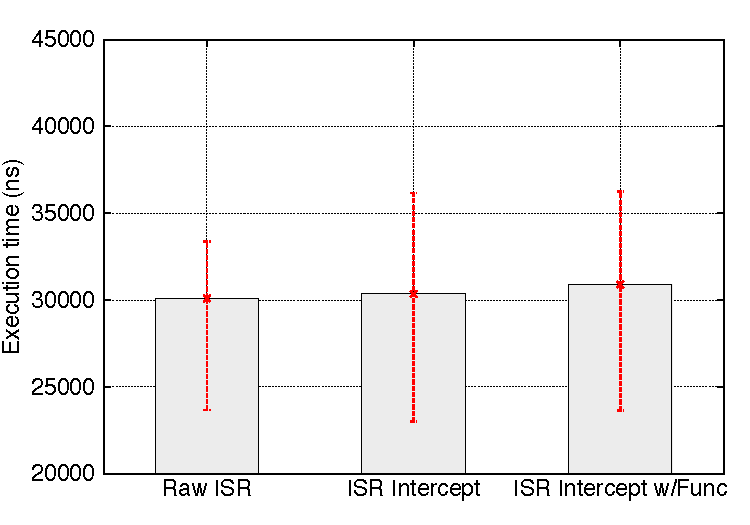
\includegraphics[width=0.4\textwidth]{graph/interrupt.pdf}
\caption{Interrupt intercept overhead}
\end{center}
\label{fig:irq_overhead}
\end{figure}

Figure \ref{irq_overhead}$B$O>e5-@_Dj$GB,Dj$7$?7k2L$G$"$k!#(B
Raw ISR$B$ODL>o$N%k!<%A%s$G<B9T$5$l$k(BISR$B!"(BISR Intercept$B$O3d$j9~$_$rEpD0$9$k$N$_!"(BISR intercept w/Func$B$OEpD0$7$?>e$G$=$N3d$j9~$_$,$I$N3d9~$_$+<1JL$7%9%1%8%e!<%i$rN)$A>e$2$k5!G=$r<B9T$7$?>l9g$G$"$k!#(B
$B$=$l$>$l(B1000$B2s$NB,Dj$GJ?6QCM$r<h$j!":G>.CM$H:GBgCM$K$D$$$F%(%i!<%P!<$G<($7$F$$$k!#(B
$B$3$N?^$+$i8+$F<h$l$k$h$&$K!"%*!<%P%X%C%I$O3N<B$KB8:_$9$k!#(B
ISR Intercept$B$@$H(B247ns$B$N%*!<%P%X%C%I$G$"$j!"(B
ISR Intercept w/Func$B$G$b(B790ns$B$N%*!<%P%X%C%I$G$"$k!#(B
$B$3$N?tCM$OD>46E*$K9M$($k$H>.$5$/%7%9%F%`<+BN$K1F6A$r5Z$\$9$[$I$G$O$J$$$H9M$($i$l$k!#(B
$B$7$+$7$=$N@Q$_=E$M$K$h$C$F$O1F6A$rM?$($k$3$H$O9M$($J$1$l$P$J$i$J$$!#(B

\subsection{Interrupt raised overhead}
$BK\9F$G$O3d9~$_N)$A>e$2$N$?$a$N%*!<%P%X%C%I$rB,Dj$9$k!#(B
$B3d9~$_N)$A>e$2$O(B2$B$D$N(BAPI$B$N8F$S=P$7$rI,MW$H$9$k!#(B
$B0l$D$O(BcuCtxCreate$B$r8F$S=P$7$?$"$H$K8F$S=P$9(Brtx\_nvrm\_init()$B$G$"$k!#(B
$B$b$&0l$D$OF14|$7$?$$%?%$%_%s%0(B(e.g. $B%+!<%M%k%i%&%s%A8e(B)$B$K8F$S=P$9(Brtx\_nvrm\_notify()$B$G$"$k!#(B
$B%9%1%8%e!<%j%s%0$r9T$o$J$$(BVanilla$B$J>uBV$G$O$3$l$i$N(BAPI$B$OI,MW$G$O$J$$$b$N$G$"$k$?$a!"$3$l$i$N(BAPI$B$K$+$+$C$?;~4V$O$9$Y$F%*!<%P%X%C%I$H$J$k!#(B

$B$=$N$?$a$3$l$i$N%*!<%P%X%C%I$N7WB,$r9T$&!#(B
$B7WB,$O(BAPI$B$N8F$S=P$7$+$iLa$k$^$G$rB,Dj$9$k!#(B

\begin{figure}[!t]
\begin{center}
\subfigure[Part of Initialize]{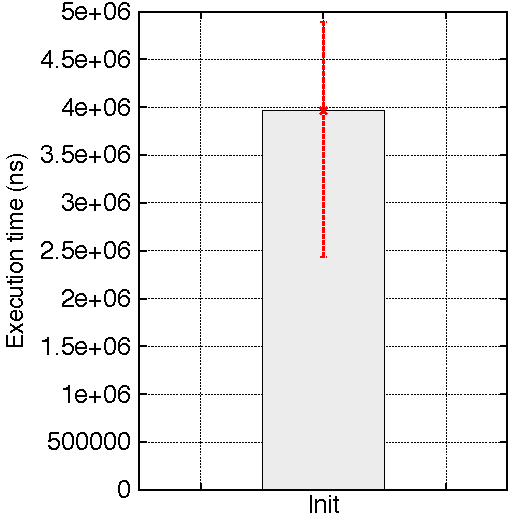
\includegraphics[width=0.23\textwidth]{graph/irq_rise_init.pdf}}\subfigure[Part of notify]{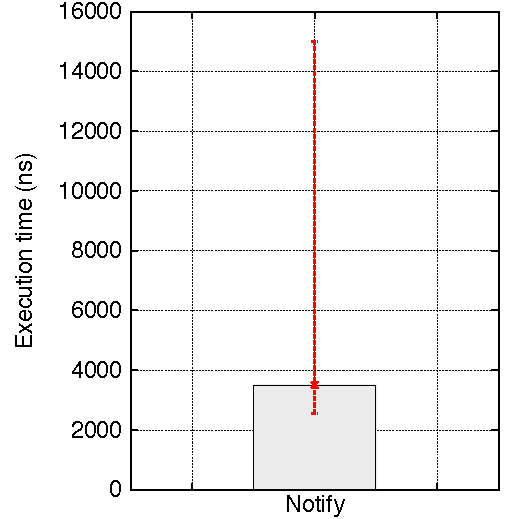
\includegraphics[width=0.23\textwidth]{graph/irq_rise_notify.pdf}}
\caption{Interrupt raised method overhead}
\label{fig:irq_rise_overhead}
\end{center}
\end{figure}

$B7k2L$r(BFigure \ref{fig:irq_rise_overhead}$B$K<($9!#(B
Initialize$B$O(BIndirect Buffer$B$O%W%m%;%9$,N)$A>e$,$k$?$S$K!"(B
$B%3%^%s%IAw?.MQ$N(BIndirect Buffer$B$N3NJ]$d3F%(%s%8%s$NEPO?$N$?$a$K8F$S=P$5$l$kI,MW$,$"$k!#(B
Notify$B$O%+!<%M%k<B9T8e$dHsF14|%a%b%j%3%T!<<B9T8e$N$h$&$J<B:]$K3d9~$_$rH/@8$5$;$?$$%?%$%_%s%0$G8F$S=P$5$l$k!#(B
$B$3$l$i$O(Bioctl$B%7%9%F%`%3!<%k$K$h$C$F%f!<%66u4V$H%+!<%M%k6u4V$r$^$?$$$G$k1F6A$+!"<B9T;~4V$N%P%iIU$-$,Bg$-$/=P$F$$$k!#(B

Initialize$B$OHf3SE*;~4V$,$+$+$C$F$$$k$,!"(B1$B%W%m%;%9$K$D$-0lEY$7$+8F$P$l$J$$$?$a!"%"%W%j%1!<%7%g%sA4BN$X$N1F6A$O>/$J$$$H9M$($i$l$k!#(B
Notify$B$K4X$7$F$O$=$l$[$I;~4V$,$+$+$C$F$*$i$:!"F14|BT$A$N4V$K<B9T$5$l$k$Y$-=hM}$J$?$a!"$3$A$i$b%"%W%j%1!<%7%g%sA4BN$X$N1F6A$O>/$J$$$H9M$($i$l$k!#(B

\subsection{Overhead}


\subsection{}


\appendices
\section{Proof of the First Zonklar Equation}
Appendix one text goes here.

% you can choose not to have a title for an appendix
% if you want by leaving the argument blank
\section{}
Appendix two text goes here.


% use section* for acknowledgement
\ifCLASSOPTIONcompsoc
  % The Computer Society usually uses the plural form
  \section*{Acknowledgments}
\else
  % regular IEEE prefers the singular form
  \section*{Acknowledgment}
\fi


The authors would like to thank...


% Can use something like this to put references on a page
% by themselves when using endfloat and the captionsoff option.
\ifCLASSOPTIONcaptionsoff
  \newpage
\fi



% trigger a \newpage just before the given reference
% number - used to balance the columns on the last page
% adjust value as needed - may need to be readjusted if
% the document is modified later
%\IEEEtriggeratref{8}
% The "triggered" command can be changed if desired:
%\IEEEtriggercmd{\enlargethispage{-5in}}

% references section

% can use a bibliography generated by BibTeX as a .bbl file
% BibTeX documentation can be easily obtained at:
% http://www.ctan.org/tex-archive/biblio/bibtex/contrib/doc/
% The IEEEtran BibTeX style support page is at:
% http://www.michaelshell.org/tex/ieeetran/bibtex/
%\bibliographystyle{IEEEtran}
% argument is your BibTeX string definitions and bibliography database(s)
%\bibliography{IEEEabrv,../bib/paper}
%
% <OR> manually copy in the resultant .bbl file
% set second argument of \begin to the number of references
% (used to reserve space for the reference number labels box)

\bibliography{IEEEabrv,bib/paper}


% biography section
% 
% If you have an EPS/PDF photo (graphicx package needed) extra braces are
% needed around the contents of the optional argument to biography to prevent
% the LaTeX parser from getting confused when it sees the complicated
% \includegraphics command within an optional argument. (You could create
% your own custom macro containing the \includegraphics command to make things
% simpler here.)
%\begin{biography}[{\includegraphics[width=1in,height=1.25in,clip,keepaspectratio]{mshell}}]{Michael Shell}
% or if you just want to reserve a space for a photo:

\begin{IEEEbiography}{Michael Shell}
Biography text here.
\end{IEEEbiography}

% if you will not have a photo at all:
\begin{IEEEbiographynophoto}{John Doe}
Biography text here.
\end{IEEEbiographynophoto}

% insert where needed to balance the two columns on the last page with
% biographies
%\newpage

\begin{IEEEbiographynophoto}{Jane Doe}
Biography text here.
\end{IEEEbiographynophoto}

% You can push biographies down or up by placing
% a \vfill before or after them. The appropriate
% use of \vfill depends on what kind of text is
% on the last page and whether or not the columns
% are being equalized.

%\vfill

% Can be used to pull up biographies so that the bottom of the last one
% is flush with the other column.
%\enlargethispage{-5in}



% that's all folks
\end{document}


